\documentclass[12pt,hyperref,a4paper,UTF8]{ctexart}
\usepackage{HDUReport}
\usepackage{listings}
\usepackage{xcolor}
\usepackage{graphicx}
\usepackage{setspace}
\usepackage{float}
\setstretch{1.5} % 设置全局行距为1.5倍

\usepackage{enumitem} % 载入enumitem包以便自定义列表环境
\setlist[itemize]{itemsep=0pt, parsep=0pt} % 设置itemize环境的项目间距和段落间距

\setmainfont{Times New Roman} % 英文正文为Times New Roman


\usepackage{tikz}
\usetikzlibrary{shapes.geometric, arrows}
\usetikzlibrary{positioning, arrows.meta}
\usetikzlibrary{calc}
%封面页设置
{   
    %标题
    \title{ 
        \vspace{1cm}
        \heiti \Huge \textbf{《电磁波与电磁场实验》作业报告} \par
        \vspace{1cm} 
        \heiti \Large {\underline{实验4：微带电路 Layout(版图)设计}   }     
    }

    \author{
        \kaishu\Large 指导教师\ \dlmu[9cm]{吴爱婷}  \\
        \kaishu\Large 学生姓名\ \dlmu[9cm]{陈文轩} \\ %学院
        \kaishu\Large 学生学号\ \dlmu[9cm]{23040447} \\ %
        \kaishu\Large 学生班级\ \dlmu[9cm]{23186011} \\ %班级
        \kaishu\Large 学生专业\ \dlmu[9cm]{智能硬件与系统(电子信息工程)} \qquad  \\ %学号
        \kaishu\Large 实验日期\ \dlmu[9cm]{2025.10.20} \qquad \\
         %姓名 
    }
        
    \date{\today} % 默认为今天的日期，可以注释掉不显示日期
}
%%------------------------document环境开始------------------------%%
\begin{document}

%%-----------------------封面--------------------%%
\cover
\thispagestyle{empty} % 首页不显示页码
%%------------------摘要-------------%%
%\newpage
%\begin{abstract}




%\end{abstract}

%\thispagestyle{empty} % 首页不显示页码

%%--------------------------目录页------------------------%%
% \newpage
% \tableofcontents
% \thispagestyle{empty} % 目录不显示页码

%%------------------------正文页从这里开始-------------------%
\newpage
\setcounter{page}{1} % 让页码从正文开始编号

%%可选择这里也放一个标题
%\begin{center}
%    \title{ \Huge \textbf{{标题}}}
%\end{center}

\section{实验目的与内容}

通过此次实验，学习如何使用Microwave Office来创建原理图的版图



\section{主要实验步骤}

\textbf{1.导入版图工艺文件(LPF)}

首先需要在Microwave Office中导入版图工艺文件，该文件定义了电路板的材料参数、介质厚度、导体层数等工艺信息。通过菜单选择Options $\rightarrow$ Layout Process File，选择对应的LPF文件进行导入，为后续的版图设计提供工艺基础。

\begin{figure}[H]
    \centering
    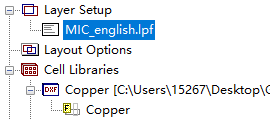
\includegraphics[width=0.8\textwidth]{figures/1.png}
    \caption{导入版图工艺文件}
\end{figure}

\textbf{2.编辑数据库单位和默认的网格大小}

在Layout Database Setup中设置数据库的单位系统和网格参数。合理的单位设置(如毫米)和网格大小可以提高版图设计的精度和效率，确保元件的精确放置和对齐。

\begin{figure}[H]
    \centering
    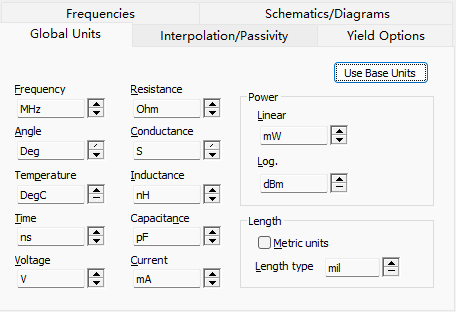
\includegraphics[width=0.8\textwidth]{figures/2.png}
    \caption{编辑数据库单位和网格大小}
\end{figure}

\textbf{3.导入版图单元库}

导入包含各种微波元件版图的单元库文件。这些单元库包含了预先设计好的无源元件(电阻、电容、电感)和传输线等的版图封装，可以直接在版图设计中调用。

\begin{figure}[H]
    \centering
    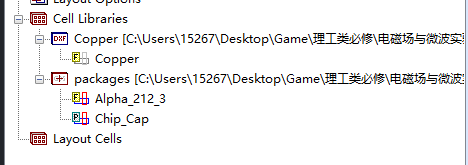
\includegraphics[width=0.8\textwidth]{figures/3.png}
    \caption{导入版图单元库}
\end{figure}

\textbf{4.在原理图中导入并放置数据文件，更改元件符号，并在版图中放置微带线完成版图}

在原理图编辑器中导入电路的网表或数据文件，根据设计需求调整元件的参数和符号。然后在版图编辑器中，使用微带线(Microstrip Line)工具绘制传输线，连接各个元件。微带线的特性阻抗$Z_0$由其宽度$W$、介质厚度$h$和相对介电常数$\varepsilon_r$决定：

$$Z_0 = \frac{87}{\sqrt{\varepsilon_r+1.41}}\ln\left(\frac{5.98h}{0.8W+T}\right)$$

其中$T$为导体厚度。

\begin{figure}[H]
    \centering
    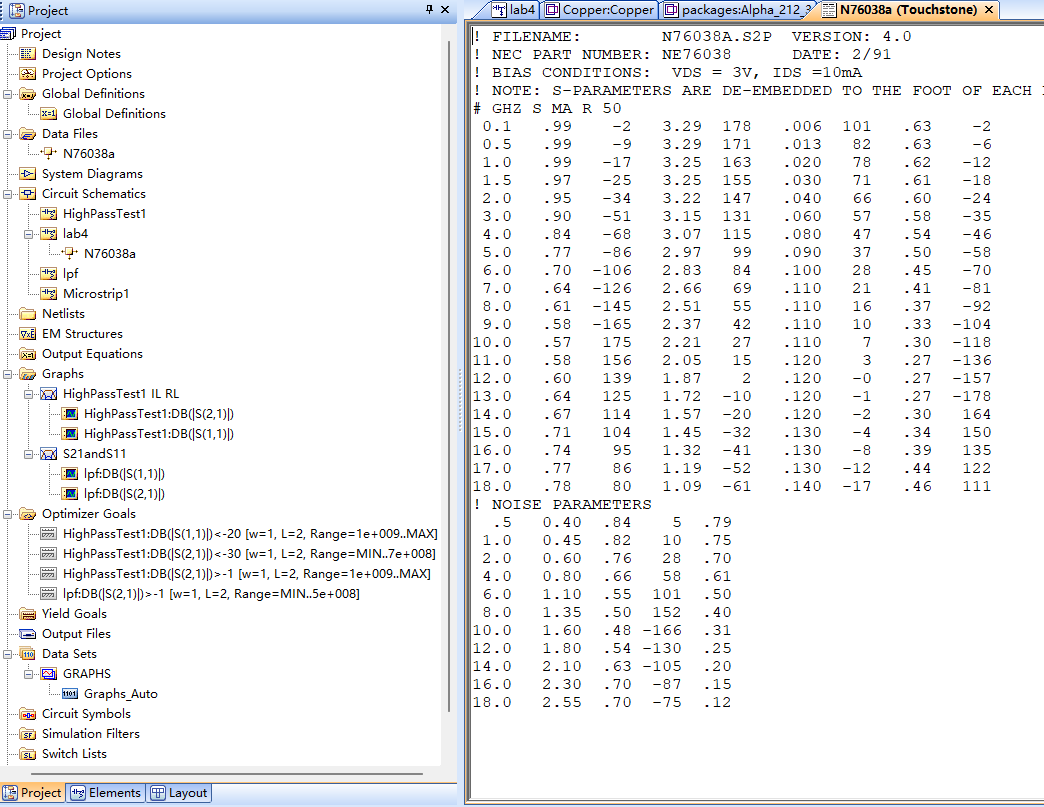
\includegraphics[width=0.7\textwidth]{figures/4.png}
    \caption{导入并放置数据文件}
\end{figure}

\begin{figure}[H]
    \centering
    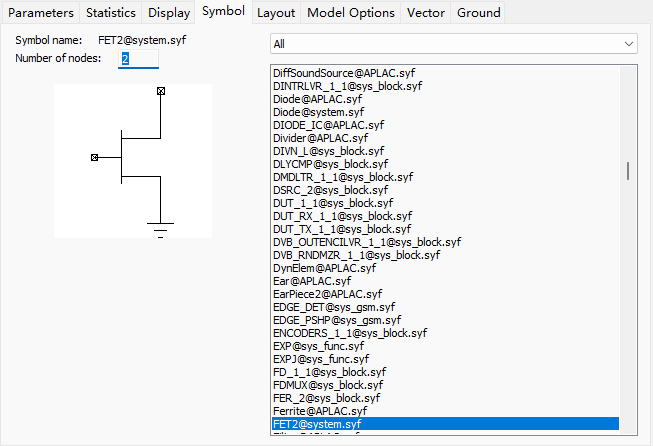
\includegraphics[width=0.7\textwidth]{figures/5.png}
    \caption{更改元件符号}
\end{figure}

\begin{figure}[H]
    \centering
    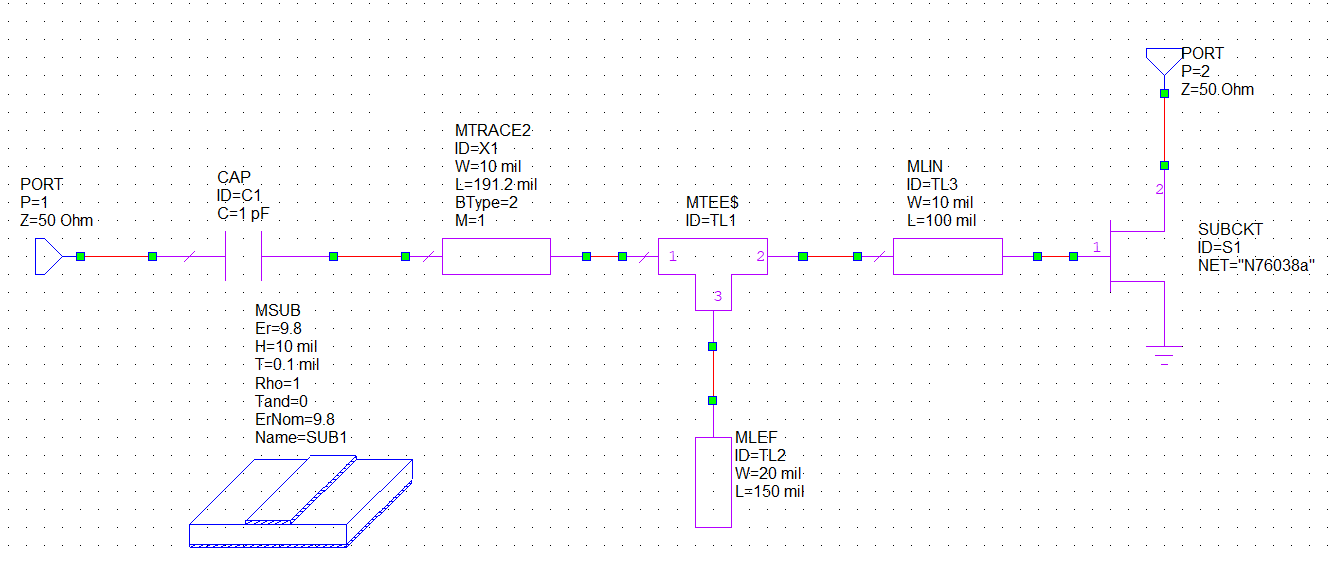
\includegraphics[width=0.7\textwidth]{figures/6.png}
    \caption{在版图中放置微带线}
\end{figure}

\textbf{5.为原理图中的元件设定封装，没有对应封装的创建封装单元}

为原理图中的每个元件指定对应的版图封装(Footprint)。如果元件库中没有合适的封装，需要手动创建新的封装单元，包括定义焊盘位置、尺寸和连接端口等信息，确保原理图与版图的一致性。

\begin{figure}[H]
    \centering
    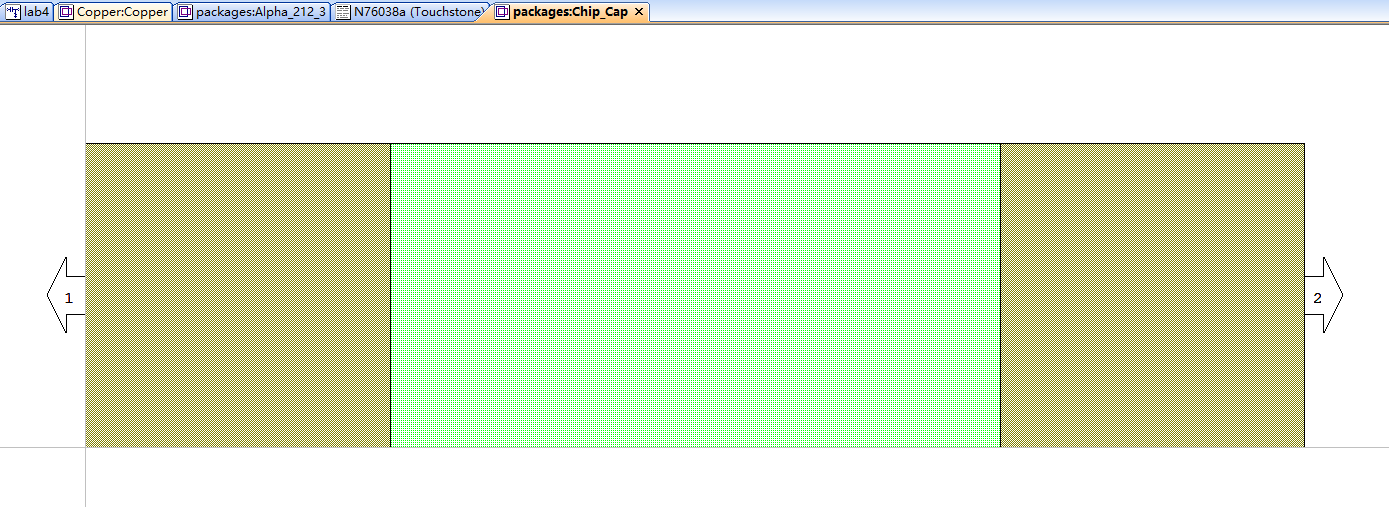
\includegraphics[width=0.8\textwidth]{figures/7.png}
    \caption{设定元件封装}
\end{figure}

\textbf{6.查看版图，使用版图的衔接功能等}

使用版图查看器检查整体布局，利用软件提供的衔接(Stitching)功能检查连接的连续性和正确性。还可以使用DRC(设计规则检查)功能验证版图是否满足工艺要求，如最小线宽、最小间距等规则。

\begin{figure}[H]
    \centering
    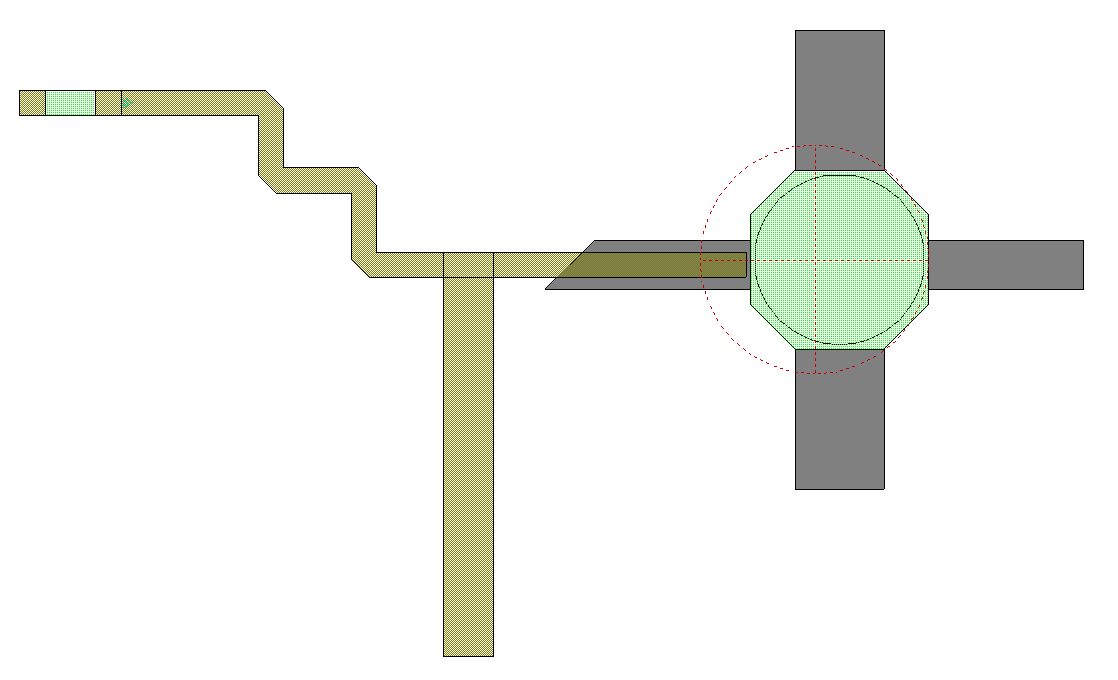
\includegraphics[width=0.8\textwidth]{figures/8.png}
    \caption{查看版图并使用衔接功能}
\end{figure}

\textbf{7.输出版图}

完成版图设计和检查后，通过File $\rightarrow$ Export导出版图文件。输出格式为DXF，这些文件可以直接用于PCB制造或进一步的EM仿真分析。

\begin{figure}[H]
    \centering
    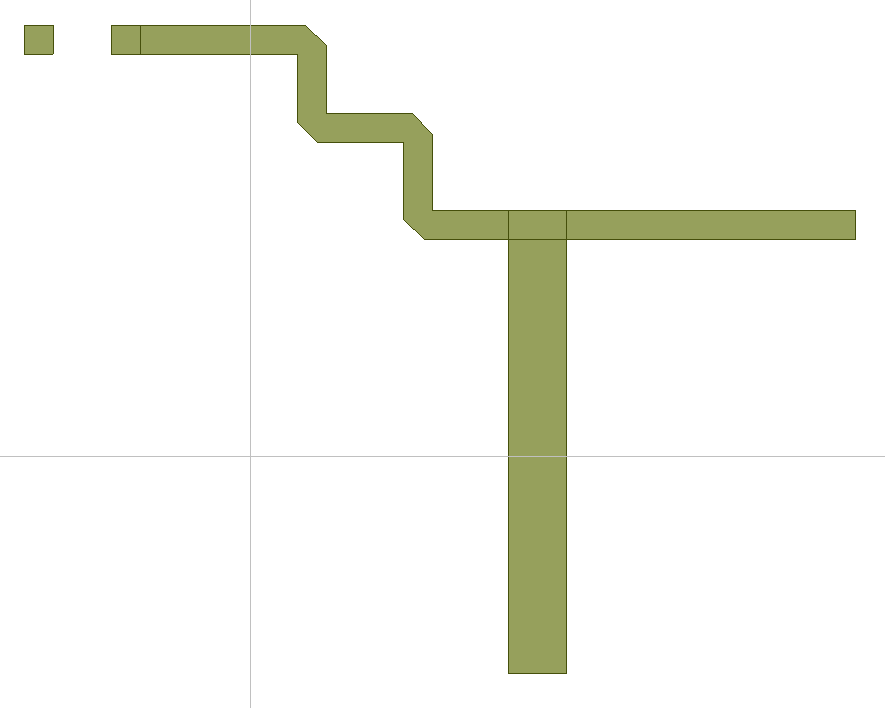
\includegraphics[width=0.8\textwidth]{figures/9.png}
    \caption{输出版图文件}
\end{figure}

\section{总结}

本次实验系统地学习了使用Microwave Office进行微波电路版图设计的完整流程。从导入工艺文件开始，初步掌握了版图数据库的设置、单元库的管理、原理图与版图的关联等关键技术。

通过实际操作，深入理解了微带线等分布参数元件的版图实现方法，以及特性阻抗与物理尺寸之间的关系。实验中学会了为元件创建封装、使用衔接功能检查连接完整性等实用技能。这些技能对于后续的微波滤波器、功分器等复杂电路的版图设计具有重要意义。

版图设计是微波电路从理论走向实践的关键环节，需要兼顾电气性能和工艺可实现性。通过本次实验，加深了对分布参数电路设计的理解，为今后的射频/微波电路设计和优化奠定了坚实的基础。同时也认识到，精确的版图设计对于保证电路性能、减少寄生效应具有至关重要的作用。




\end{document}